\documentclass[a4paper,11pt]{article}

\usepackage[french]{babel}
\usepackage[utf8]{inputenc}
\usepackage[left=2.5cm,top=2cm,right=2.5cm,nohead,nofoot]{geometry}
\usepackage{url}
\usepackage{graphicx}
\usepackage{hyperref}
\usepackage{listings}
\usepackage{amsmath}
\usepackage{amssymb}
\usepackage{color}
\usepackage{listings}
\usepackage{graphicx}
\usepackage{float}
\usepackage{todonotes}
\setcounter{section}{-1}




\linespread{1.1}



\begin{document}

\begin{titlepage}
\begin{center}
\textbf{\textsc{UNIVERSIT\'E LIBRE DE BRUXELLES}}\\
\textbf{\textsc{Faculté des Sciences}}\\
\textbf{\textsc{Département d'Informatique}}
\vfill{}\vfill{}
\begin{center}{\Huge Projet : Logique Propositionnelle et Utilisation de l’Outil MiniSat}\end{center}{\Huge \par}
\begin{center}{\large Pierre Gérard, Antoine Carpentier}\end{center}{\Huge \par}
\vfill{}\vfill{} \vfill{}
\begin{flushleft}{\large \textbf{INFO-F-302 Informatique Fondamentale}}\hfill{Emmanuel FILIOT, Guillermo Pérez}\end{flushleft}{\large\par}
\vfill{}\vfill{}\enlargethispage{3cm}
\textbf{Année académique 2014~-~2015}
\end{center}
\end{titlepage}

%\begin{abstract}
%Ce rapport présente ...
%\end{abstract}


\tableofcontents

\pagebreak

\section{Introduction}

\subsection{Tester l'implémentation}
Pour testez facilement l'ensemble de nos implémentation, utilisez le script bash disponible de la manière suivante :
\begin{lstlisting}
$ sh TestMe.sh	
\end{lstlisting}
Ce bash script va faire le build, et exécuter minisat avec des inputs choisis en fonction de la question.

\subsection{Parser}
Pour le parser, nous avons décidé de ne pas utiliser l'ensemble du code du parser fournit. Nous avons donc seulement gardé la classe ShedSpec en créant nous même la structure de donnée nécessaire pour son constructeur.

\section{Q1}
Les contraintes sont les suivantes :
\begin{itemize}
  \item Contrainte d'existence : chaque examen se déroule dans au moins une salle et durant au moins une période de temps,
  \item Le nombre d'étudiant dans une salle ne peut pas dépasser sa capacité,
  \item Un étudiant ne peut pas avoir deux examens au même moment,
  \item Un professeur ne peut pas avoir deux examens au même moment,
  \item Un examen doit avoir au moins un professeur,
  \item Un examen doit avoir au moins un étudiant
  \item Chaque examen doit se dérouler exactement une seule fois,
  \item Chaque examen doit se dérouler exactement dans une seule salle,
  \item Dans une salle, il ne peut se déroule qu'un seul examen a la fois.
\end{itemize}


\section{Q2}
\subsection{Contrainte d'existence : chaque examen se déroule dans au moins une salle et durant au moins une période de temps}
\begin{displaymath}
	\forall x \in X, \exists s \in S, \exists t \in T : \mu(x) = (s,t) 
\end{displaymath}

\subsection {Le nombre d'étudiant dans une salle ne peut pas dépasser sa capacité}
\begin{displaymath}
\forall x \in X , \forall s \in S ,\forall e \in E, \forall t \in \{1,...,T\} : \mu(x) = (s,t) \Rightarrow (\sum a(e) \mapsto \{x\}) \leq c(s)
\end{displaymath}	

\subsection {Un étudiant ne peut pas avoir deux examens au même moment}
\begin{displaymath}
\forall x_{1},x_{2} \in X, \forall s_{1},s_{2} \in S , \forall e \in E ,\forall t_{1}, t_{2} \in \{1,...,T\} :  x_{1} \neq x_{2} \wedge a(e) \mapsto \{x_{1},x_{2}\}  \wedge \mu(x_{1}) = (s_{1},t_{1}) \wedge\end{displaymath}
\begin{displaymath}
 \mu(x_{2}) = (s_{2},t_{2}) \Rightarrow t_{1} \neq t_{2} 
\end{displaymath}

\subsection {Un professeur ne peut pas avoir deux examens au même moment}
\begin{displaymath}
\forall x_{1},x_{2} \in X, \forall s_{1},s_{2} \in S , \forall p \in P ,\forall t_{1}, t_{2} \in \{1,...,T\} :  x_{1} \neq x_{2} \wedge b(p) \mapsto \{x_{1},x_{2}\}  \wedge \mu(x_{1}) = (s_{1},t_{1}) \wedge\end{displaymath}
\begin{displaymath}
 \mu(x_{2}) = (s_{2},t_{2}) \Rightarrow t_{1} \neq t_{2} 
\end{displaymath}

\subsection {Un examen doit avoir au moins un professeur}
\begin{displaymath}
\forall x \in X, \exists p \in P : b(p) \mapsto \{x\} 
\end{displaymath}

\subsection {Un examen doit avoir au moins un étudiant}
\begin{displaymath}
\forall x \in X, \exists e \in E : a(e) \mapsto \{x\}
\end{displaymath}

\subsection {Chaque examen doit se dérouler une seule fois}
\begin{displaymath}
\forall t_{1}, t_{2} \in \{1,...,T\},\forall s_{1},s_{2} \in S, \forall x \in X : \mu(x) = (s_{1},t_{1}) \wedge \mu(x) = (s_{2},t_{2}) \Rightarrow t_{1} = t_{2}
\end{displaymath}

\subsection {Chaque examen doit se dérouler dans une seule salle}
\begin{displaymath}
\forall t_{1}, t_{2} \in \{1,...,T\},\forall s_{1},s_{2} \in S, \forall x \in X : \mu(x) = (s_{1},t_{1}) \wedge \mu(x) = (s_{2},t_{2}) \Rightarrow s_{1} = s_{2}
\end{displaymath}

\subsection {Dans une salle, il ne peut se dérouler qu'un seul examen a la fois}
\begin{displaymath}
\forall t \in \{1,...,T\},\forall x_{1},x_{2} \in X, \forall s \in S : \mu(x_{1}) = (s,t) \wedge \mu(x_{2}) = (s,t) \Rightarrow x_{1} = x_{2}
\end{displaymath}	

\section{Q3}
Pour construire la formule en FNC, nous avons besoins de définir de nouvelles variables.
\begin{itemize}
    \item \(E\) est le nombre d'étudiants,
    \item \(P\) est le nombre de professeurs,
    \item \(X\) est le nombre d'examens,
    \item \(S\) est le nombre de salles,
    \item \(T\) est le nombre de périodes de temps,
	\item \( A_{e,x}\) telle que l'étudiant e passe l'examen x,
	\item \(B_{p,x}\) telle que le professeur p donne l'examen x ,
	\item \(C_{s,i}\) telle que la salle s a la capacité d'accueillir i étudiants,
	\item \(N_{x}\) telle que la fonction N donne le nombre d'étudiant qui passe l'examen x.
\end{itemize}


\subsection{Ensemble de FNC}
\subsubsection{(p1)}
Contrainte d'existence : chaque examen se déroule dans au moins une salle et durant au moins une période de temps.
Il s'agit de dire qu'il existe au moins une proposition valable pour chaque examen, quel que soit la période de temps ou salle.
\begin{displaymath}
	\bigwedge\limits_{x=1}^{X}\bigvee\limits_{s=1}^{S}\bigvee\limits_{t=1}^{T} M_{s,x,t}
\end{displaymath}


\subsubsection{(p2)}
Le nombre d'étudiant dans une salle ne peut pas dépasser sa capacité.
Il s'agit de dire qu'une proposition n'est pas valable pour chaque examen et chaque période de temps si la salle n'a pas la capacité d'accepter le nombre d'étudiants ayant cet examen.
\begin{displaymath}
	\bigwedge\limits_{t=1}^{T}\bigwedge\limits_{x=1}^{X}\bigwedge\limits_{\substack{s=1 \\ \neg C_{s,N_{x}}}}^{S}  \neg M_{x,s,t}
\end{displaymath}

\subsubsection{(p3)}
Un étudiant ne peut pas avoir deux examens au même moment.
Il s'agit de dire qu'il existe au maximum une proposition valable pour tous les examens de chaque étudiant se déroulant au même moment, quelle que soit la salle.
\begin{displaymath}
\bigwedge\limits_{e=1}^{E}\bigwedge\limits_{t=1}^{T}\bigwedge\limits_{s_{1}=1}^{S}\bigwedge\limits_{s_{2}=1}^{S}\bigwedge\limits_{\substack{x1=1 \\ A_{e,x_{1}}}}^{X}\bigwedge\limits_{\substack{x_{2}=x_{1}+1 \\ A_{e,x_{2}}}}^{X} \neg M_{x_{1}, s_{1}, t} \vee \neg M_{x_{2}, s_{2}, t}
\end{displaymath}

\subsubsection{(p4)}
Un professeur ne peut pas avoir deux examens au même moment.
Il s'agit de dire qu'il existe au maximum une proposition valable pour tous les examens de chaque professeur se déroulant au même moment, quelle que soit la salle.
\begin{displaymath}
\bigwedge\limits_{p=1}^{P}\bigwedge\limits_{t=1}^{T}\bigwedge\limits_{s_{1}=1}^{S}\bigwedge\limits_{s_{2}=1}^{S}\bigwedge\limits_{\substack{x_{1}=1 \\ B_{p,x_{1}}}}^{X}\bigwedge\limits_{\substack{x_{2}=x_{1}+1 \\ B_{p,x_{2}}}}^{X} \neg M_{x_{1}, s_{1}, t} \vee \neg M_{x_{2}, s_{2}, t}
\end{displaymath}

\subsubsection{(p5)}
Un examen doit avoir au moins un professeur.
Il s'agit de dire qu'il existe au minimum une proposition valable pour chaque examen quelque soit la salle ou la période de temps telle qu'un professeur donne cet examen.
\begin{displaymath}
\bigwedge\limits_{x=1}^{X}\bigvee\limits_{s=1}^{S}\bigvee\limits_{t=1}^{T}\bigvee\limits_{\substack{p=1 \\ B_{p,x}}}^{P} M_{x, s, t}
\end{displaymath}

\subsubsection{(p6)}
Un examen doit avoir au moins un étudiant.
Il s'agit de dire qu'il existe au minimum une proposition valable pour chaque examen quelque soit la salle ou la période de temps telle qu'un étudiant passe cet examen.
\begin{displaymath}
\bigwedge\limits_{x=1}^{X}\bigvee\limits_{s=1}^{S}\bigvee\limits_{t=1}^{T}\bigvee\limits_{\substack{e=1 \\ A_{e,x}}}^{E} M_{x, s, t}
\end{displaymath}

\subsubsection{(p7)}
Chaque examen doit se dérouler une seule fois.
Il s'agit de dire qu'il existe au maximum une proposition valable pour chaque examen pour chaque temps quelle que soit la salle.
\begin{displaymath}
\bigwedge\limits_{x=1}^{X}\bigwedge\limits_{s=1}^{S}\bigwedge\limits_{t_{1}=1}^{T}\bigwedge\limits_{t_{2}=t_{1}+1}^{T} \neg M_{x, s, t_{1}} \vee \neg M_{x, s, t_{2}}
\end{displaymath}

\subsubsection{(p8)}
Chaque examen doit se dérouler dans une seule salle.
Il s'agit de dire qu'il existe au maximum une proposition valable pour chaque examen pour chaque salle quelle que soit la période de temps.
\begin{displaymath}
\bigwedge\limits_{x=1}^{X}\bigwedge\limits_{t=1}^{T}\bigwedge\limits_{s_{1}=1}^{S}\bigwedge\limits_{s_{2}=t1+1}^{S} \neg M_{x, s_{1}, t} \vee \neg M_{x, s_{2}, t}
\end{displaymath}

\subsubsection{(p9)}
Dans une salle, il ne peut se déroule qu'un seul examen a la fois.
Il s'agit de dire qu'il existe au maximum une proposition valable pour chaque salle pour chaque examen quelle que soit la période de temps.
\begin{displaymath}
\bigwedge\limits_{s=1}^{S}\bigwedge\limits_{t=1}^{T}\bigwedge\limits_{x_{1}=1}^{X}\bigwedge\limits_{x_{2}=t1+1}^{X} \neg M_{x_{1}, s, t} \vee \neg M_{x_{2}, s, t}
\end{displaymath}

\subsection{Note}
La redondance n'est pas un problème car MiniSat supprime les doublons de clauses.

\subsection{FNC final}
La forme normal conjonctive de la formule est:
\begin{displaymath}
\Phi_{I} = p1 \wedge p2 \wedge p3 \wedge p4 \wedge p5 \wedge p6 \wedge p7 \wedge p8 \wedge p9
\end{displaymath}

\section{Q4}

\subsection{Exemple de résultat}
Nous avons créé une liste d'input possible pour cette question. Voici quelque exemple
\subsubsection{Construction d'un horaire possible}
Input fournis avec l'énoncé.
\begin{lstlisting}[
    basicstyle=\tiny, %or \small or \footnotesize etc.
]
$ ./projq4.out "4 ;3 ;10 ;30 ;100 ;100 ;2 ;4 ;1; 1; 1 ;1 ;1 ;1 ;1 ;1 ;1 ;1 ;1 ;1 ;1 ;1 ;1 ;1 ;1 ;1 ;1 ;1
 ;1 ;1 ;1 ;1 ;1 ;1 ;1 ;1 ;1 ;1 ;2 ;2 ;2 ;2 ;2 ;2 ;2 ;2 ;2 ;2 ;2 ;2 ;2 ;2 ;2 ;2 ;2 ;2 ;2 ;2 ;2 ;2 ;2 ;2 
 ;2 ;2 ;2 ;2 ;2 ;2 ;3,4 ;3,4 ;3,4 ;3,4 ;3,4 ;3,4 ;3,4 ;3,4 ;3,4 ;3,4 ;3,4 ;3,4 ;3,4 ;3,4 ;3,4 ;3,4 
 ;3,4 ;3,4 ;3,4 ;3,4 ;3,4 ;3,4 ;3,4 ;3,4 ;3,4 ;3,4 ;3,4 ;3,4 ;3,4 ;3,4 ;3,4 ;3,4 ;3,4 ;3,4 ;3,4 ;3,4 
 ;3,4 ;3,4 ;3,4 ;3,4 ;1,3 ;2,4;
---------------------------------------- Result ----------------------------------------
T = 4
|S| = 3
c(s1) = 10
c(s2) = 30
c(s3) = 100
|E| = 100
|P| = 2
|X| = 4
a(e1) = { 1 }
[...]
a(e30) = { 1 }
[...]
a(e60) = { 2 }
a(e61) = { 3 4 }
[...]
a(e99) = { 3 4 }
a(e100) = { 3 4 }
b(p1) = { 1 3 }
b(p2) = { 2 4 }
==================================[MINISAT]===================================
| Conflicts |     ORIGINAL     |              LEARNT              | Progress |
|           | Clauses Literals |   Limit Clauses Literals  Lit/Cl |          |
==============================================================================
|         0 |     260     3528 |      86       0        0     nan |  0.000 % |
==============================================================================
Success, the problem has been solve under those constraints !
Examen 1 dans la salle 2 au temps 1
Examen 2 dans la salle 2 au temps 2
Examen 3 dans la salle 3 au temps 2
Examen 4 dans la salle 3 au temps 1

OUTPUT : 2,1;2,2;3,2;3,1;
\end{lstlisting}

\subsubsection{Construction d'un horaire impossible}
Input créé de tel manière qu'il n'y ait pas moyen de construire un horaire.
\begin{lstlisting}[
    basicstyle=\tiny, %or \small or \footnotesize etc.
]
$ ./projq4.out "1 ;3 ;1 ;10 ;50 ;2 ;2 ;2 ;1,2 ;1 ;1 ;2 ;"
---------------------------------------- Result ----------------------------------------
T = 1
|S| = 3
c(s1) = 1
c(s2) = 10
c(s3) = 50
|E| = 2
|P| = 2
|X| = 2
a(e1) = { 1 2 }
a(e2) = { 1 }
b(p1) = { 1 }
b(p2) = { 2 }
==================================[MINISAT]===================================
| Conflicts |     ORIGINAL     |              LEARNT              | Progress |
|           | Clauses Literals |   Limit Clauses Literals  Lit/Cl |          |
==============================================================================
|         0 |      18       53 |       6       0        0     nan |  0.000 % |
==============================================================================
Uh .. The problem could not be solve under those constraints

OUTPUT : 0
\end{lstlisting}

\section{Q5}

\subsection{Hypothèses}
Pour cette question et les prochaines, nous considérons qu'une période de temps dure 1h.

\subsection{Nouvelle variable}

Pour construire la formule en FNC, nous avons besoins de définir une nouvelle variable :  
\begin{itemize}
	\item \( D_{x}\) qui donne la durée de l'examen x.
\end{itemize}

A la question numéro 4, dans les contraintes, nous avons considéré que les examens durent une seule période de temps. Nous devons donc en modifier certaines pour prendre en compte le fait que un examen dure plusieurs périodes de temps. 
Le principe des deux contraintes qui suivent ainsi que de la nouvelle contrainte consiste à admettre au maximum un examen parmi deux si ils leurs horaires se chevauchent. Pour deux examens se déroulant respectivement aux temps $t1$ et $t2$ et de durées respectivement $d1$ et $d2$, la condition pour qu'ils se chevauchent est : 
\begin{align}
t1 <= t2 + d2 \wedge t2 <= t1 + d1
\iff \neg (t1 > t2 + d2 \vee t2 < t1 + d1)
\end{align}

\subsection{Modification de contrainte}

\subsubsection{Un étudiant ne peut pas avoir deux examens au même moment}
Cette contrainte autorise pour chaque étudiant au maximum un examen parmi deux avec des temps différents qui se chevauchent.\\
(p3)
\begin{displaymath}
\bigwedge\limits_{e=1}^{E}\bigwedge\limits_{t1=1}^{T}\bigwedge\limits_{\substack{t2=1 \\ t1 <= t2 + D(x2)-1 \wedge t1 + D(x1)-1 >= t2}}^{T}\bigwedge\limits_{s=1}^{S}\bigwedge\limits_{\substack{x1=1 \\ A_{e,x1}}}^{X}\bigwedge\limits_{\substack{x2=x1+1 \\ A_{e,x2}}}^{X} \neg M_{x1, s1, t_{1}} \vee \neg M_{x2, s2, t_{2}}
\end{displaymath}

\subsubsection{Un professeur ne peut pas avoir deux examens au même moment}
Cette contrainte autorise pour chaque professeur au maximum un examen parmi deux avec des temps différents qui se chevauchent.\\
(p4)
\begin{displaymath}
\bigwedge\limits_{p=1}^{P}\bigwedge\limits_{t1=1}^{T}\bigwedge\limits_{\substack{t2=1 \\ t1 <= t2 + D(x2)-1 \wedge t1 + D(x1)-1 >= t2}}^{T}\bigwedge\limits_{s=1}^{S}\bigwedge\limits_{\substack{x1=1 \\ B_{p,x1}}}^{X}\bigwedge\limits_{\substack{x2=x1+1 \\ B_{p,x2}}}^{X} \neg M_{x1, s1, t_{1}} \vee \neg M_{x2, s2, t_{2}}
\end{displaymath}

\subsubsection{Chaque examen doit avoir le temps de se dérouler}
On modifie la contrainte (p7) devenue inutile car la contrainte ci-dessous assure que chaque examen se déroulera dans un nombre de périodes de temps exactement égal à sa durée. Par contre il n'y aucune garantie qu'un examen aura assez de temps pour se dérouler si il commence proche de la dernière période de temps. On empêche donc l'examen $x$ de se dérouler dans une période de temps après $ T - D_{x} + 1 $.\\
(p7)
\begin{displaymath}
\bigwedge\limits_{x=1}^{X}\bigwedge\limits_{s=1}^{S}\bigwedge\limits_{t=T - D_{x} + 1}^{T} \neg M_{x, s, t}
\end{displaymath}


\subsection{Nouvelle contrainte}

\subsubsection{Chaque examen doit avoir un nombre de période de de temps égal à sa durée et ses périodes de temps doivent être continues}
Pour modéliser la durée d'un examen il a fallut penser le problème autrement. En effet nous avons considéré un examen commençant à une certaine période et durant un certain temps. Nous devons ensuite vérifier que chaque examen existe dans chaque salle sans chevaucher un autre examen (expliqué ci-dessus), ce qui vérifie alors la contrainte de durée.\\

(p10)
\begin{displaymath}
\bigwedge\limits_{x_{1}=1}^{X}\bigwedge\limits_{\substack{x_{2}=1 \\ x_{1} \neq x_{2}}}^{X}\bigwedge\limits_{s=1}^{S}\bigwedge\limits_{t_{1}=1}^{T}\bigvee\limits_{\substack{t_{2}=0 \\ t_{1} < t_{2} + D(x_{2})-1 \wedge t_{1} + D(x_{1})-1 > t_{2}}}^{T} \neg M_{x_{1}, s, t_{1}} \vee \neg M_{x_{2}, s, t_{2}}
\end{displaymath}

\subsection{FNC}
Pour obtenir la nouvelle FNC final, on prend en compte les modifications de contrainte et on rajoute la nouvelles.

\begin{displaymath}
	\Phi_{D} = p1 \wedge p2 \wedge p3 \wedge p4 \wedge p5 \wedge p6 \wedge p7 \wedge p8 \wedge p9 \wedge p10
\end{displaymath}

\subsection{Exemple de résultats}
Voici un exemple avec 3 salles, 100 étudiants, 2 professeur.
\begin{lstlisting}[
    basicstyle=\tiny, %or \small or \footnotesize etc.
]
$ ./projq5.out "12 ;3 ;10 ;30 ;100 ;100 ;2 ;4 ;1; 1; 1 ;1 ;1 ;1 ;1 ;1 ;1 ;1 ;1 ;1 ;1 ;1 ;1 ;1 ;1 ;1 ;
1 ;1 ;1 ;1 ;1 ;1 ;1 ;1 ;1 ;1 ;1 ;1 ;2 ;2 ;2 ;2 ;2 ;2 ;2 ;2 ;2 ;2 ;2 ;2 ;2 ;2 ;2 ;2 ;2 ;2 ;2 ;2 ;2 ;2 ;
2 ;2 ;2 ;2 ;2 ;2 ;2 ;2 ;3,4 ;3,4 ;3,4 ;3,4 ;3,4 ;3,4 ;3,4 ;3,4 ;3,4 ;3,4 ;3,4 ;3,4 ;3,4 ;3,4 ;3,4 ;
3,4 ;3,4 ;3,4 ;3,4 ;3,4 ;3,4 ;3,4 ;
3,4 ;3,4 ;3,4 ;3,4 ;3,4 ;3,4 ;3,4 ;3,4 ;3,4 ;3,4 ;3,4 ;3,4 ;3,4 ;3,4 ;3,4 ;3,4 ;3,4 ;3,4 ;1,3 ;
2,4; 2; 4; 2; 3;"

---------------------------------------- Result ----------------------------------------
T = 12
|S| = 3
c(s1) = 10
c(s2) = 30
c(s3) = 100
|E| = 100
|P| = 2
|X| = 4
a(e1) = { 1 }
[...]
a(e30) = { 1 }
a(e31) = { 2 }
[...]
a(e60) = { 2 }
a(e61) = { 3 4 }
[...}
a(e99) = { 3 4 }
a(e100) = { 3 4 }
b(p1) = { 1 3 }
b(p2) = { 2 4 }
d(x1) = 2
d(x2) = 4
d(x3) = 2
d(x4) = 3
==================================[MINISAT]===================================
| Conflicts |     ORIGINAL     |              LEARNT              | Progress |
|           | Clauses Literals |   Limit Clauses Literals  Lit/Cl |          |
==============================================================================
|         0 |    1868    36217 |     622       0        0     nan |  0.000 % |
==============================================================================
Success, the problem has been solve under those constraints !
Examen 1 dans la salle 2 au temps 1
Examen 2 dans la salle 2 au temps 4
Examen 3 dans la salle 3 au temps 4
Examen 4 dans la salle 3 au temps 1

OUTPUT : 2,1;2,4;3,4;3,1;

\end{lstlisting}
On remarque que le résultat est cohérent. En effet, les durée sont prise en compte et les différents examens des professeurs et des élèves aussi. Exemple comme le professeur 2 à l'examen 2 et 4, le 2 ne commence que en temps 4 alors que la salle 2 est libre dès le temps 3.

\section{Q6}

\subsection{Hypothèse}
Pour cette question, nous avons supposé que les examens se déroulaient tous les jours de 8h à 20h. L'ensemble de paires de périodes où les examens ne sont pas possibles ont été codés dans la classe SchedSpec sous la variable I. Notre implémentation permet de les modifiers sans avoir à modifier le reste du code.
En supposant que les périodes de temps commencent à minuit le premier jour des examens, nous avons interdit les périodes entre les numéros 1 et 8 compris, 21 et 32 compris et ainsi de suite en ajoutant 24 (la durée d'un jour en heure) jusqu'à la fin des périodes de temps.

\subsection{Nouvelle variable}

Pour construire la formule en FNC, nous avons besoins de définir une nouvelle variable :  
\begin{itemize}
	\item \( J_{t}\) tel que $t$  ne trouve pas dans les périodes de nuit, donc qu'il est possible d'avoir un examen en période $t$.
\end{itemize}

\subsection{Modification de contrainte}
Aucune contrainte déjà existante n'a du être modifiée pour ce problème.

\subsection{Nouvelle contrainte}

\subsubsection{Aucun examen ne peut se dérouler durant certains intervalles de temps}
(p11)
\begin{displaymath}
\bigwedge\limits_{x_{1}=1}^{X}\bigwedge\limits_{s=1}^{S}\bigwedge\limits_{\substack{t=0 \\ \neg J(t) }}^{T} \neg M_{x, s, t}
\end{displaymath}

\subsection{FNC}
\begin{displaymath}
	\Phi_{N} = p1 \wedge p2 \wedge p3 \wedge p4 \wedge p5 \wedge p6 \wedge p7 \wedge p8 \wedge p9 \wedge p10 \wedge p11
\end{displaymath}
\subsection{Exemple de résultats}
20 examens, durée variant de 1 à 4 et 1 à 4 examen par étudiant.

\begin{lstlisting}[
    basicstyle=\tiny, %or \small or \footnotesize etc.
]
$ ./projq6.out "100;10;100;150;147;49;154;174;62;164;121;181;100;10;20;20,7,19;17,7,2;10,11,15;13,4,19;6,9,11;
17,8,5;17,8,16;20,2,1;15,11,6;4,4,19;11,10,9;6,13,16;3,17,10;2,6,11;16,19,12;5,13,9;20,11,15;7,9,13;
14,2,3;5,15,11;2,2,16;14,10,18;16,4,1;6,19,4;6,19,7;11,11,20;16,15,20;14,20,8;13,20,9;8,6,6;4,17,7;
15,3,16;17,15,19;10,10,4;7,14,9;10,6,6;4,11,1;15,3,2;16,9,8;18,5,11;6,18,20;13,13,3;1,10,1;15,6,19;
3,1,15;10,2,6;7,19,11;13,18,18;4,19,1;17,12,1;9,5,8;11,16,1;19,12,4;2,8,2;6,14,6;10,13,6;11,14,10;
9,17,19;6,2,2;9,5,11;10,11,8;20,13,3;11,1,6;13,4,9;12,6,12;7,5,13;15,7,2;17,18,13;13,8,9;7,16,3;
18,2,17;4,13,19;5,15,6;3,19,7;10,15,13;19,18,6;9,9,10;20,14,9;20,19,20;17,4,1;4,12,18;17,11,15;
13,8,15;5,3,20;12,15,7;9,2,15;3,11,16;1,7,2;6,14,1;8,9,20;19,9,16;12,16,16;5,15,9;20,19,16;4,20,20;
3,1,18;3,18,8;17,1,9;14,13,13;6,1,13;2,7,3,16,1;12,11,15,13,18;5,8,2;6,6,19,20,10;5;14,1,20,5;
4,4,5,7,8;6,15,10,17,9;1,9;20,16,2,1;4;1;1;4;4;1;1;4;1;4;1;4;2;2;4;3;2;3;3;3;"

==================================[MINISAT]===================================
| Conflicts |     ORIGINAL     |              LEARNT              | Progress |
|           | Clauses Literals |   Limit Clauses Literals  Lit/Cl |          |
==============================================================================
|         0 | 6020540 12069760 | 2006846       0        0    -nan |  0.000 % |
==============================================================================
Success, the problem has been solve under those constraints !
Examen 1 dans la salle 1 au temps 81
Examen 2 dans la salle 1 au temps 14
Examen 3 dans la salle 1 au temps 42
Examen 4 dans la salle 1 au temps 67
Examen 5 dans la salle 1 au temps 63
Examen 6 dans la salle 1 au temps 62
Examen 7 dans la salle 1 au temps 61
Examen 8 dans la salle 1 au temps 57
Examen 9 dans la salle 1 au temps 17
Examen 10 dans la salle 1 au temps 44
Examen 11 dans la salle 1 au temps 43
Examen 12 dans la salle 1 au temps 39
Examen 13 dans la salle 1 au temps 37
Examen 14 dans la salle 1 au temps 19
Examen 15 dans la salle 1 au temps 33
Examen 16 dans la salle 1 au temps 20
Examen 17 dans la salle 1 au temps 18
Examen 18 dans la salle 1 au temps 15
Examen 19 dans la salle 1 au temps 12
Examen 20 dans la salle 1 au temps 9
 
OUTPUT : 1,81;1,14;1,42;1,67;1,63;1,62;1,61;1,57;1,17;1,44;1,43;1,39;1,37;1,19;1,33;1,20;1,18;1,15;1,12;1,9;
\end{lstlisting}
Dans cet exemple on voit bien les périodes de temps sans examens correspondant aux nuits.
\section{Q7}
\subsection{Nouvelle contrainte}
\subsubsection{La somme, pour tout étudiant e, du nombre de changements de salle de e, est bornée par k}
Pour cette contrainte il nous faut trouver toutes possibilités d'examens et de salles dans l'ordre chronologique pour chaque étudiant. Ainsi, pour chaque possiblité, on peut déterminer si le nombre de changement de salles est plus grand k. Dans ce cas, on invalide la proposition.
(p12)
\begin{displaymath}
	TODO	
\end{displaymath}

\subsection{FNC}
\begin{displaymath}
	\Phi_{N} = p1 \wedge p2 \wedge p3 \wedge p4 \wedge p5 \wedge p6 \wedge p7 \wedge p8 \wedge p9 \wedge p10 \wedge p11 \wedge p12
\end{displaymath}
	
\subsection{Implémentation}
\subsection{Exemple de résultats}

\section{Q8}

Nous n'avons pas réussi a utiliser le module Max-Sat de MiniSat.
En effet, aucune documentation n'était disponible.

Cependant, avec notre implémentation actuel nous pourrions minimiser k. Cela suivrait le pseudo code suivant :

\begin{lstlisting}[
    basicstyle=\tiny, %or \small or \footnotesize etc.
]
	for k in range(X):
		problem.solve(k)
		if problem.solved:
			print "Ce probleme peut etre modeliser avec une valeur de k = " + k
			break
\end{lstlisting}
Evidemment, ce n'est pas une manière optimal de minimiser une variable.

\section{Q9}

\subsection{Modification de contrainte}
\subsubsection{Les examens d'un étudiant ne se chevauchent pas}
On reprend la contrainte défini dans la q5 et on la divise en deux cas. 

Le premier est lorsque deux salles sont identique. Dans ce cas on modifie la durée tel que il y ait une période en plus.
(p3a)
\begin{displaymath}
\bigwedge\limits_{e=1}^{E}\bigwedge\limits_{t1=1}^{T}\bigwedge\limits_{\substack{t2=1 \\ t1 <= t2 + D(x2) \wedge t1 + D(x1) >= t2}}^{T}\bigwedge\limits_{s_{1}=1}^{S}\bigwedge\limits_{\substack{s2=1 \\ s_{1} \neq s_{2}}}^{S}\bigwedge\limits_{\substack{x1=1 \\ A_{e,x1}}}^{X}\bigwedge\limits_{\substack{x2=x1+1 \\ A_{e,x2}}}^{X} \neg M_{x1, s1, t} \vee \neg M_{x2, s2, t}
\end{displaymath}
(p3b)
Dans le deuxième cas, si les salles sont identique, on fait comme a la question 5.
\begin{displaymath}
\bigwedge\limits_{e=1}^{E}\bigwedge\limits_{t1=1}^{T}\bigwedge\limits_{\substack{t2=1 \\ t1 <= t2 + D(x2)-1 \wedge t1 + D(x1)-1 >= t2}}^{T}\bigwedge\limits_{s_{1}=1}^{S}\bigwedge\limits_{\substack{s2=1 \\ s_{1} = s_{2}}}^{S}\bigwedge\limits_{\substack{x1=1 \\ A_{e,x1}}}^{X}\bigwedge\limits_{\substack{x2=x1+1 \\ A_{e,x2}}}^{X} \neg M_{x1, s1, t} \vee \neg M_{x2, s2, t}
\end{displaymath}

$ (p3) = (p3a) \wedge (p3b) $
\subsection{FNC}
\begin{displaymath}
	\Phi_{N} = p1 \wedge p2 \wedge p3 \wedge p4 \wedge p5 \wedge p6 \wedge p7 \wedge p8 \wedge p9 \wedge p10 \wedge p11 \wedge p12
\end{displaymath}
\subsection{Implémentation}
\subsection{Exemple de résultats}

\begin{lstlisting}[
    basicstyle=\tiny, %or \small or \footnotesize etc.
]
$ ./projq9.out "20 ;3 ;10 ;30 ;100 ;10 ;5 ;5 ; 1,3;3;4;5;1,2;1,2;1,2;1,2;1,2;1,2;1;2;3;4;5;4;3;2;3;4;2;"
---------------------------------------- Result ----------------------------------------
T = 20
|S| = 3
c(s1) = 10
c(s2) = 30
c(s3) = 100
|E| = 10
|P| = 5
|X| = 5
a(e1) = { 1 3 }
a(e2) = { 3 }
a(e3) = { 4 }
a(e4) = { 5 }
a(e5) = { 1 2 }
a(e6) = { 1 2 }
a(e7) = { 1 2 }
a(e8) = { 1 2 }
a(e9) = { 1 2 }
a(e10) = { 1 2 }
b(p1) = { 1 }
b(p2) = { 2 }
b(p3) = { 3 }
b(p4) = { 4 }
b(p5) = { 5 }
d(x1) = 4
d(x2) = 3
d(x3) = 2
d(x4) = 3
d(x5) = 4
==================================[MINISAT]===================================
| Conflicts |     ORIGINAL     |              LEARNT              | Progress |
|           | Clauses Literals |   Limit Clauses Literals  Lit/Cl |          |
==============================================================================
|         0 |    4884    18906 |    1628       0        0     nan |  0.000 % |
==============================================================================
Success, the problem has been solve under those constraints !
Examen 1 dans la salle 2 au temps 9
Examen 2 dans la salle 1 au temps 15
Examen 3 dans la salle 1 au temps 14
Examen 4 dans la salle 1 au temps 12
Examen 5 dans la salle 1 au temps 9

OUTPUT : 2,9;1,15;1,14;1,12;1,9;

\end{lstlisting}
Dans cette exemple on voit que l'étudiant 1 à l'examen 1 et 3 dans deux salles différentes. Il y a bien durée(examen 1) + une unité de temps entre les deux.

\section{Q10}
\subsection{Certains examens dans certaines salles (ex. salle informatique)}
Pour modéliser la contrainte, nous avons besoins de définir une nouvelle variable :  
\begin{itemize}
	\item \( XS_{x,s}\) tel que l'examen x peut se dérouler dans la salle s.
\end{itemize}
\begin{displaymath}
	\bigwedge\limits_{x=1}^{X}\bigwedge\limits_{\substack{s=1 \\ \neg XS(x,s)}}^{S}\bigwedge\limits_{t=1}^{T} \neg M_{x, s, t} 
\end{displaymath}


\subsection{Si deux examens se suivent et sont sur des campus différents, il y a 2 temps entre ces deux examens}
Pour modéliser la contrainte, nous avons besoins de définir une nouvelle variable :  
\begin{itemize}
	\item \( SC_{s1,s2}\) tel que s1 est sur un campus différent de s2.
\end{itemize}
Pou réaliser cela, nous devons modifier la contrainte p3 (pas d'examen qui se chevauche) : 

(p3a) Pas de changement de salle
\begin{displaymath}
\bigwedge\limits_{e=1}^{E}\bigwedge\limits_{t1=1}^{T}\bigwedge\limits_{\substack{t2=1 \\ t1 <= t2 + D(x2)-1 \wedge \\ t1 + D(x1)-1 >= t2}}^{T}\bigwedge\limits_{s_{1}=1}^{S}\bigwedge\limits_{\substack{s2=1 \\ s_{1} = s_{2}}}^{S}\bigwedge\limits_{\substack{x1=1 \\ A_{e,x1}}}^{X}\bigwedge\limits_{\substack{x2=x1+1 \\ A_{e,x2}}}^{!X} \neg M_{x1, s1, t} \vee \neg M_{x2, s2, t}
\end{displaymath}

(p3b) Changement de salle mais pas de campus
\begin{displaymath}
\bigwedge\limits_{e=1}^{E}\bigwedge\limits_{t1=1}^{T}\bigwedge\limits_{\substack{t2=1 \\ t1 <= t2 + D(x2) \wedge \\ t1 + D(x1) >= t2}}^{T}\bigwedge\limits_{s_{1}=1}^{S}\bigwedge\limits_{\substack{s2=1 \\ s_{1} \neq s_{2} \wedge \neg SC_{s1,s2} }}^{S}\bigwedge\limits_{\substack{x1=1 \\ A_{e,x1}}}^{X}\bigwedge\limits_{\substack{x2=x1+1 \\ A_{e,x2}}}^{X} \neg M_{x1, s1, t} \vee \neg M_{x2, s2, t}
\end{displaymath}

(p3c) Changement de salle et de campus
\begin{displaymath}
\bigwedge\limits_{e=1}^{E}\bigwedge\limits_{t1=1}^{T}\bigwedge\limits_{\substack{t2=1 \\ t1 <= t2 + D(x2) +1 \wedge \\ t1 + D(x1) +1 >= t2}}^{T}\bigwedge\limits_{s_{1}=1}^{S}\bigwedge\limits_{\substack{s2=1 \\ s_{1} \neq s_{2} \wedge SC_{s1,s2}}}^{S}\bigwedge\limits_{\substack{x1=1 \\ A_{e,x1}}}^{X}\bigwedge\limits_{\substack{x2=x1+1 \\ A_{e,x2}}}^{X} \neg M_{x1, s1, t} \vee \neg M_{x2, s2, t}
\end{displaymath}


$ (p3) = (p3a) \wedge (p3b) \wedge (p3c)$


\section{Q11}
Pour rappel, voici les différentes complexités P, NP, NP-complet et NP-dur.
\begin{figure}[H]
  \centering
  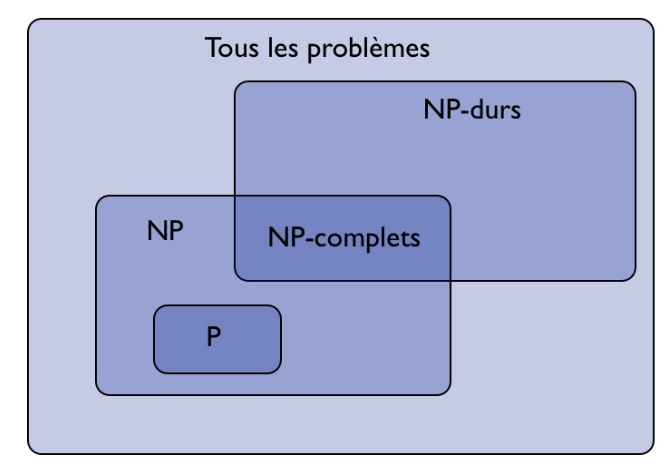
\includegraphics[scale=0.4]{images/q11-p-np-nphardcomplete.png}
  \caption{\label{} P, NP, NP-complet et NP-dur}
\end{figure}
Pour prouver qu'un problème est NP-dur, il faut montrer qu'un problème NP-dur connu peut se ramener à notre problème en temps polynômial.

Nous allons donc montrer que le problème \textbf{Job Shop Scheduling with Sequence-Dependent Setup} peut se réduire à notre problème d'emploi du temps en temps polynômial. Le problème de Job Shop Scheduling with Sequence-Dependent Setup est NP-dur \footnote{Artigues, Christian, Sana Belmokhtar, and Dominique Feillet. "A new exact solution algorithm for the job shop problem with sequence-dependent setup times." \textit{Integration of ai and or techniques in constraint programming for combinatorial optimization problems}. Springer Berlin Heidelberg, 2004. 37-49.}.

On pose les jobs comme étant des examens, les machines comme étant des salles allouables aux examens, la durée d'un job comme étant la durée d'un examen et on garde les périodes de temps. Dans une machine (salle), il ne peut pas y avoir deux jobs (examens) en même temps. Chaque job (examen) doit se dérouler exactement une fois et avec exactement une machine (salle).
La fonction de coût des machines peut être modélisée avec la capacité des salles dans notre problème.
Les contraintes externes empêchant certains jobs de s'exécuter en même temps (Sequence-Dependent Setup) sont similaires au fait que les examens que passent un étudiant et ceux que donnent un professeur ne peuvent pas se dérouler en même temps peuvent être modélisée comme une matrix $ N x N $ de valeurs booléennes dans les deux cas (N étant le nombre d'examens ou de jobs), indiquant si deux jobs (examens) peuvent se dérouler en même temps ou non.
Le but de notre problème puisqu'il faut effectuer tous les examens dans une certaine période de temps T et donc minimiser le temps total, ce qui est le cas également pour le \textbf{Job Shop Scheduling with Sequence-Dependent Setup} où il faut minimiser le temps total des jobs.
\end{document}

